\section{Present Muon Trigger}

\subsection{Global Trigger Data-Flow}

Each of the three muon detector systems in CMS participates in the Level-1 (L1) muon trigger for coverage and redundancy. For the DT and CSC systems ($|\eta|$ $<$ 1.2 and $|\eta|$ $>$ 0.9, respectively), the front-end trigger primitive generator (TPG) electronics identify track segments from the hit information registered in multiple gas planes of a single measurement station. These segments are collected and then transmitted via optical fibres to regional Track-Finders in the electronics service cavern, which then apply pattern recognition algorithms in order to identify muon candidates and measure their momenta from the magnetic bending in the return yoke between several measurement stations. Information is shared between the DT Track-Finder (DTTF) and CSC Track-Finder (CSCTF) for efficient coverage in the region of overlap between the two systems at $|\eta|$ $\approx 1$. The hits from the RPC system ($|\eta|<1.6$) are directly sent from the front-end electronics to Pattern Comparator (PAC) logic boards that identify muon candidates.

The three regional track-finders sort the identified muon candidates and transmit to the Global Muon Trigger (GMT) up to 4 (CSCTF, DTTF) or 8 (RPC) candidates every bunch crossing. Each candidate has been assigned a $p_T$ and quality code as well as $\eta$ and $\phi$ positions in the muon system (with a granularity of $\approx 0.05$). The GMT then merges muon candidates found by more than one system to eliminate fake multi-muon triggers (with several options on how to select $p_T$ between the candidates), and can suppress muon candidates in some regions of the detector if their quality is low and they are unconfirmed by another muon detector system. The data flow of the present L1 muon trigger is shown in Fig.~\ref{fig:l1_muon_trig}.

\begin{figure}[b]
	\begin{center}
		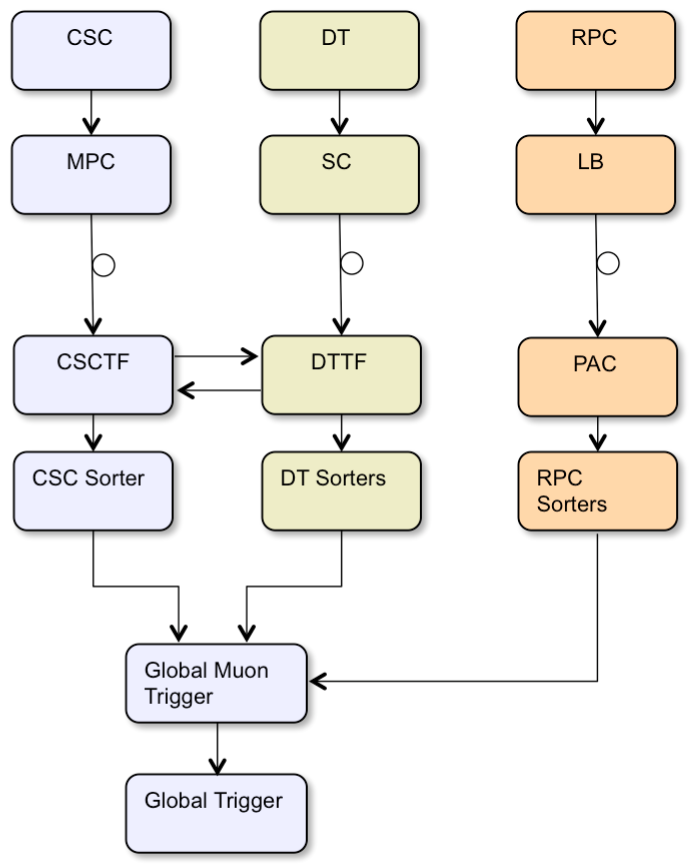
\includegraphics[width=0.48\linewidth]{figures/dataflow_current_L1_trigger.png}
	\end{center}
	\caption{Data-flow of the present L1 muon trigger. \label{fig:l1_muon_trig} }
\end{figure}

\subsection{Muon Trigger in Endcaps}

Each CSC can provide up to two local charged track (LCT) segments to the trigger logic per bunch crossing (BX, where 1 BX = 25 ns). These are formed in the trigger motherboard (TMB) combining cathode (CLCT) and anode (ALCT) segments. Present and improved logics of the algorithm which constructs LCTs are described in Section~\ref{sec:present_algo} and Section~\ref{sec:SLHC_algo}, respectively. The CLCT data contains information on the azimuthal position of the segment ($\phi$), the bend angle, and the pattern of cathode half-strips with hits in a chamber. The ALCT data contains information on the radial position from the beamline of the segment (equivalent to $\eta$), and the pattern of anode wires with hits in a chamber. The timing information from anodes is used to define the time of the combined LCT. There is one TMB per CSC, located in a crate on the periphery of the detector. The TMB sends up to two LCTs over a custom backplane to the muon port card (MPC), which is located in the same peripheral crate. One MPC can receive data from up to 9 TMBs, or equivalently, can receive up to 18 LCTs. The LCTs in a MPC are sorted by rank (see definition in MPC documentation). The best three LCTs are sent over optical fibers to the CSCTF. There are a total of sixty peripheral crates for the CSC system, each with one MPC.

The CSCTF system is partitioned into sectors, each of which corresponds to a $60^{o}$ azimuthal region of an endcap. Twelve ``sector processors'' are required for the entire endcap muon system, six per endcap. Each sector processor is a 9U VME card that is housed in a single crate. Three 1.6 Gb/s optical links from each of five MPCs are received by each sector processor, for a total of 180 optical links for the entire system. The CSCTF sectors are independent, since there is no sharing of data across boundaries of neighboring sectors, leading to slight inefficiencies.

There are several Field Programmable Gate Arrays (FPGAs) on each ``sector processor'', but the main FPGA for the track-finding algorithms is from the Xilinx Virtex-5 family. The conversion of strip and wire positions of each track segment to ($\eta, \phi$) coordinates is accomplished via a set of cascaded SRAM look-up tables (LUTs), each $512K\times16$ bits. These coordinates are then used for track-finding and momentum assignment.

The CSCTF track-finding logic consists of pairwise comparisons of track segments in different detector stations. These test for compatibility in $\phi$ and $\eta$ with a muon emanating from the collision vertex within certain tolerance windows. The comparisons are then analyzed and built into tracks consisting of possibly more than two segments from different stations. Possible duplicate (“ghost”) tracks are canceled. The track-finding logic has the ability to accept segments in different assigned bunch crossings by analyzing across a sliding time window of programmable length (nominally 2 BX) every bunch crossing. Duplicate tracks found on consecutive bunch crossings are canceled. The bunch crossing of a track is given by the second arriving track segment.

The $p_T$ of a muon candidate is calculated by using a large LUT implemented in SRAM. Information such as the track type, track $\eta$, the segment $\phi$ differences between a maximum of 3 stations, and the segment bend angle in the first measurement station are used to calculate the LUT address.

In addition to identifying muons from proton collisions, the CSCTF processors also simultaneously identifies any beam halo muons for monitoring and veto purposes by looking for trajectories approximately parallel to the beam line.

Each CSCTF sends up to three muon candidates per bunch crossing over a custom backplane to a muon sorter (MS). The MS then sorts the candidates by momentum and quality and selects the best 4 for the GMT. The CSCTF data are also sent to a DAQ card with SLINK interface which puts the trigger data into the event record.
